% siminos/atlas/symm.tex  pdflatex atlas
% $Author$ $Date$


% \section{What is a symmetry?}
% \label{s:symm}

% \section{Dynamics and symmetries: a recap}
% \label{s:cutting}


    \ifdraft\color{blue}
{\large Das Problem}
Drifting is energetically cheap.
Flows are lazy, rather than do work, solutions drift along non-shape-changing
symmetry directions.
Symmetry-preserving, non-shape changing  drifts are cheap, as they are not
shape changing and burn no energy


    \color{black}\fi


\begin{figure}
\begin{center}
  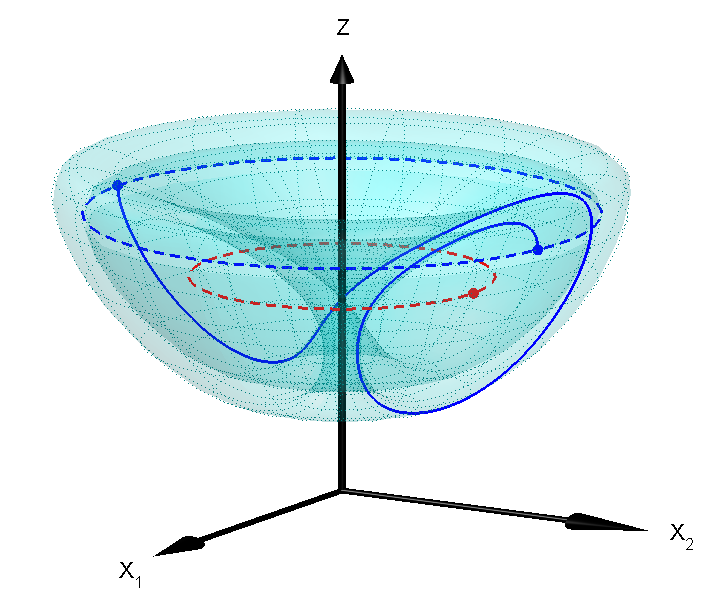
\includegraphics[width=0.35\textwidth,clip=true]{01grouporbit}
\end{center}
  \caption
  [\CLf: $\cycle{01}$ {\rpo} group orbit]{
  \CLf: The \reqv\ $\REQV{}{1}$ is shown by the red dot, and the dashed
  red line is its group orbit / trajectory. One period of the
  $\cycle{01}$ {\rpo} is shown by the solid blue line. The group orbit of
  its (arbitrary) starting point is shown by the dashed blue line: after
  one period the trajectory has returned to the group orbit but with a
  different phase. The group orbit of the $\cycle{01}$ trajectory (dark
  blue) is shown by the cyan surface. Trajectory of the further 15
  repeats of $\cycle{01}$ (faint dotted lines) traces out ergodically the
  torus generated by the$\cycle{01}$  group.
  }
\label{fig:CLf01group}
\end{figure}


\subsection{Pipes and planes}

 %% A27*-pipeSymms.* - read dasbuch/book/FigSrc/inkscape/00ReadMe.txt
 \begin{figure}
 \begin{center}
  \setlength{\unitlength}{0.20\textwidth}
  %% \unitlength = units used in the Picture Environment
(a)
  \begin{picture}(1,0.52454249)%
    \put(0,0){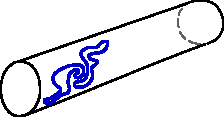
\includegraphics[width=\unitlength]{A27a-pipeSymms}}%
    \put(0.61583231,0.13683004){\color[rgb]{0,0,0}\makebox(0,0)[lb]{\smash{$z$}}}%
    \put(0.00611823,0.27217453){\color[rgb]{0,0,0}\makebox(0,0)[lb]{\smash{$\theta$}}}%
  \end{picture}%
(b)
  \begin{picture}(1,0.52454249)%
    \put(0,0){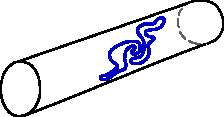
\includegraphics[width=\unitlength]{A27b-pipeSymms}}%
    \put(0.61583231,0.13683004){\color[rgb]{0,0,0}\makebox(0,0)[lb]{\smash{$z$}}}%
    \put(0.00611823,0.27217453){\color[rgb]{0,0,0}\makebox(0,0)[lb]{\smash{$\theta$}}}%
  \end{picture}%
\\
(c)
  \begin{picture}(1,0.52454249)%
    \put(0,0){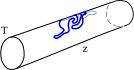
\includegraphics[width=\unitlength]{A27c-pipeSymms}}%
    \put(0.61583231,0.13683004){\color[rgb]{0,0,0}\makebox(0,0)[lb]{\smash{$z$}}}%
    \put(0.00611823,0.27217453){\color[rgb]{0,0,0}\makebox(0,0)[lb]{\smash{$\theta$}}}%
  \end{picture}%
(d)
  \begin{picture}(1,0.52454249)%
    \put(0,0){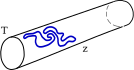
\includegraphics[width=\unitlength]{A27d-pipeSymms}}%
    \put(0.61583231,0.13683004){\color[rgb]{0,0,0}\makebox(0,0)[lb]{\smash{$z$}}}%
    \put(0.00611823,0.27217453){\color[rgb]{0,0,0}\makebox(0,0)[lb]{\smash{$\theta$}}}%
  \end{picture}%
 \end{center}
 \caption{\label{fig:A27-pipeSymms}
$\On{2}_\theta \times \SOn{2}_z$ symmetry of flow in a stream-wise
periodic pipe: A \rpo\ $p$ is a state of the fluid
 (a)
that reappears
 (b)
period $\period{}$ later, translated by downstream shift $\shift$
(in contrast to a \reqv, a constant shape that travels
downstream with constant {\phaseVel} $\velRel$); such solutions are
stream-wise $\SOn{2}_z$ equivariant; or
 (c)
period $\period{}$ later, translated by downstream shift $\shift$ and
rotated azimuthaly by $\gSpace_p$; $\SOn{2}_{\theta} \times \SOn{2}_z$
equivariant; or
 (d)
period $\period{}$ later, reflected and rotated azimuthaly by
$\gSpace$; $\On{2}_{\theta}$ equivariant
(from \wwwcb{}).
 }%
 \end{figure}
													\toCB
    \PC{emphasize that our turbulent states are \emph{not} localized
    three-dimensional solitary waves as quasi-particles -
    \reffig{fig:A27-pipeSymms} might be misleading. Our solutions are
    global, distributed over the whole volume.}
The symmetry group $\Gpipe$ of stream-wise periodic pipe flow contains
two commuting \SOn{2} rotations (\reffig{fig:A27-pipeSymms}). Each
\SOn{2} group orbit is topologically a circle
(\reffig{fig:2840GOt135th0}), and together they sweep out a contorted
$T^2$ torus (\reffig{fig:2830GO6}).

\subsection{\CLe}

As an example, consider the $\SOn{2}$-equivariant Gibbon and
McGuinness\rf{GibMcCLE82,FowlerCLE82} \cLe\
\bea
	\dot{x}_1 &=& -\sigma x_1 + \sigma y_1\continue
	\dot{x}_2 &=& -\sigma x_2 + \sigma y_2\continue
	\dot{y}_1 &=& (\RerCLor-z) x_1 - \ImrCLor x_2 -y_1-e y_2 \continue
	\dot{y}_2 &=& \ImrCLor x_1 + (\RerCLor-z) x_2 + e y_1- y_2\continue
	\dot{z} \; &=& -b z + x_1 y_1 + x_2 y_2
    \,.
\label{eq:CLeR}
\eea
For the background and an in-depth investigation in present context, see
\refrefs{SiminosThesis}. In all examples considered here, the parameters
are set to Siminos values $\RerCLor=28,\, \ImrCLor=0,\, b=8/3,\,
\sigma=10,\, e= 1/10$.

%%%%%%%%%%%%%%%%%%%%%%%%%%%%%%%%%%%%%%%%%%%%%%%%%
% 2011-09-09, 2012-03-30 Predrag: add BeThMovFr to
%            continuous.tex overheads, and ChaosBook
% replace A27movFrame*.* everywhere
\begin{figure}
 \begin{center}
  \setlength{\unitlength}{0.20\textwidth}
  %% \unitlength = units used in the Picture Environment
(a)~~
  \begin{picture}(1,0.98655417)%
    \put(0,0){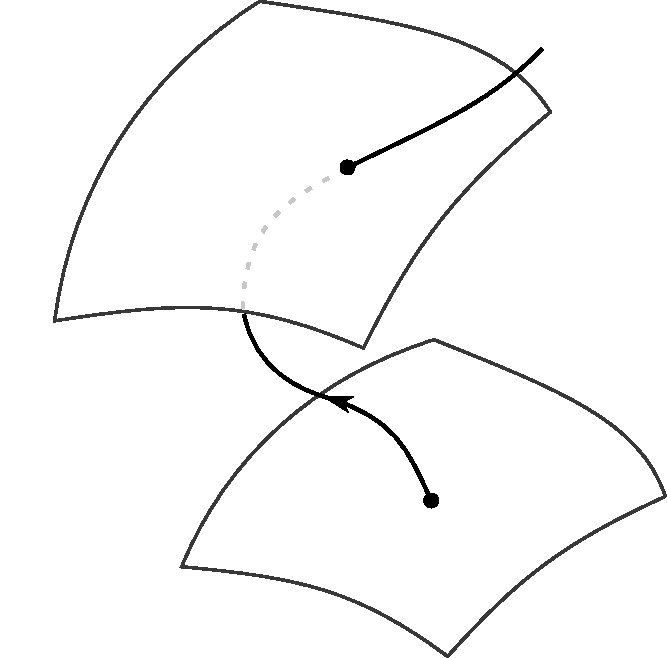
\includegraphics[width=\unitlength]{BeThTrajTeX}}%
    \put(0.35976094,0.91875614){\color[rgb]{0,0,0}\rotatebox{-31.32889204}{\makebox(0,0)[lb]{\smash{$\pS_{\ssp(\zeit)}$}}}}%
        \put(0.60333631,0.42274457){\color[rgb]{0,0,0}\rotatebox{-40.8073288}{\makebox(0,0)[lb]{\smash{$\pS_{\ssp(0)}$}}}}%
    \put(0.66001383,0.16959019){\color[rgb]{0,0,0}\rotatebox{0.0313674}{\makebox(0,0)[lb]{\smash{$\ssp(0)$}}}}%
    \put(0.5058276,0.64524238){\color[rgb]{0,0,0}\rotatebox{0.0313674}{\makebox(0,0)[lb]{\smash{$\ssp(\zeit)$}}}}%
    \put(0.13110825,0.05766516){\color[rgb]{0,0,0}\rotatebox{0.11031334}{\makebox(0,0)[lb]{\smash{$\pS$}}}}%
  \end{picture}%
~~(b)
  \begin{picture}(1,0.98655417)%
    \put(0,0){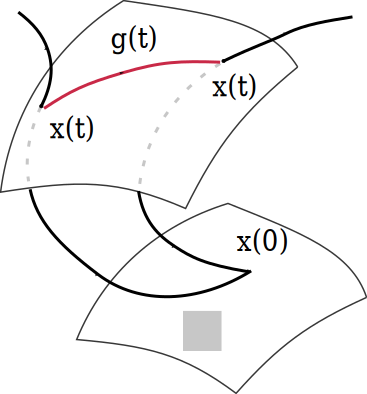
\includegraphics[width=\unitlength]{BeThMovFr}}%
    \put(0.20559239,0.64023845){\color[rgb]{0,0,0}\rotatebox{0.0313674}{\makebox(0,0)[lb]{\smash{$\ssp(\zeit)$}}}}%
    \put(0.67382401,0.35781161){\color[rgb]{0,0,0}\rotatebox{0.0313674}{\makebox(0,0)[lb]{\smash{$\ssp(0)$}}}}%
    \put(0.61221026,0.74589514){\color[rgb]{0,0,0}\rotatebox{0.0313674}{\makebox(0,0)[lb]{\smash{$\sspRed(\zeit)$}}}}%
    \put(0.35760559,0.8662057){\color[rgb]{0,0,0}\rotatebox{0.0313674}{\makebox(0,0)[lb]{\smash{$\LieEl(\zeit)$}}}}%
  \end{picture}%
 \end{center}
  \caption{\label{fig:BeThMovFr}
(a)
The group orbit $\pS_{\ssp(0)}$ of \statesp\ point $\ssp(0)$, and the
group orbit $\pS_{\ssp(\zeit)}$ reached by the trajectory $\ssp(\zeit)$ time $t$
later.
(b)
The two physically equivalent flows $\ssp(\zeit)=\LieEl(\zeit)\,\sspRed(\zeit)$ are related
by, in general, an arbitrary, time dependent {\em moving frame} transformation $\LieEl(\zeit)$.
(from \wwwcb{}).
  }
\end{figure}
%%%%%%%%%%%%%%%%%%%%%%%%%%%%%%%%%%%%%%%%%%%%%%%%%%

\subsection{Relative invariant solutions}
\label{s:RelInvSol}

An example of a wurst is the set of group orbits traced out by a single
short \rpo\ in \reffig{fig:CLf01group}. As \cLe\ exhibits only the simplest,
$m=1$ Fourier mode, all group orbits are circles, which appear elliptical in
most $d=5 \to 3$~dimensions projections.

A {\em \reqv} is a dynamical
orbit whose velocity field
lies within the group tangent space, with a constant phase velocity $c$,
% $c=(c_1,\cdots,c_N)$,
and whose time evolution is thus confined to the group orbit, \ie,
\(
\vel(\ssp) = c \cdot \groupTan(\ssp)
\) %\label{phaseVel}\\
%\ssp(\zeit) &=& \LieEl(\gSpace(\zeit)) \, \ssp(0)
%          = \mathrm{e}^{ \zeit  c \Lg} \,  \ssp(0)
%           = \mathrm{e}^{ \zeit\,  c \cdot \Lg} \,  \ssp(0)
%\,,\qquad
%\ssp(\zeit) \in \pS_{\REQV{}{}}
%\nnu
%\,.
%\eea
Depending on the context, \reqva\ can also be called traveling waves and
rotational waves.
A {\rpo} $p$ is an orbit in {\statesp} $\pS$ which exactly recurs
\[ %beq
\ssp(\zeit) = \LieEl_p \, \ssp(\zeit + \period{p} )
    \,,\qquad
\ssp(\zeit) \in \pS_p
\] %ee{RPOrelper1}
after a fixed {relative period} $\period{p}$, but shifted by a fixed
group action ${\LieEl}$ that maps the endpoint $\ssp (\period{}) $ back
into the initial point cycle point $\ssp (0) $ (see the pipe flow
sketches \reffig{fig:A27-pipeSymms} and \reffig{fig:CLf01group} for an
example in \CLf).
